\documentclass[xcolor=dvipsnames]{beamer}
\usepackage{beamerthemesplit}
%\usepackage{natbib}
\usepackage{bm,amsmath,color}
\definecolor{darkblue}{rgb}{0.0,0.0,0.50}
\definecolor{myorange}{cmyk}{0,0.7,1,0}
\hypersetup{colorlinks = true, linkcolor=darkblue, citecolor=darkblue, 
urlcolor=darkblue}
\hypersetup{pdfauthor={A. Richards}, pdftitle={De Oliveria Martins \& Posada}}

%% links
%\let\oldcite=\cite                                                              
%\renewcommand{\cite}[1]{darkblue}{\oldcite{#1}}}
%\renewcommand{\cite}[1]{\textcolor[rgb]{0.0,.7,1.0}{\oldcite{#1}}}

\newcommand{\rd}{\textcolor {red}}
\newcommand{\highlt}{\textcolor {myorange}}
\def\ci{\perp\!\!\!\perp}
%% set beamer theme and color
\usetheme{Frankfurt}
%\usecolortheme{dolphin}
\usecolortheme{rose}
\setbeamertemplate{blocks}[rounded][shadow=true]

%% beamer packages
% other themes: AnnArbor, Antibes, Bergen, Berkeley, Berlin, Boadilla, boxes, 
% CambridgeUS, Darmstadt, Dresden, Frankfurt, Goettingen, Hannover, Ilmenau,
%JuanLesPins, Luebeck, Madrid, Malmoe, Marburg, Montpellier, PaloAlto,
%Pittsburgh, Rochester, Singapore, Szeged, Warsaw
% other colors: albatross, beaver, crane, default, dolphin, dove, fly, lily, 
%orchid, rose, seagull, seahorse, sidebartab, structure, whale, wolverine,
%beetle
\title[Discussion]{A Bayesian Supetree Model for Genome-Wide Species Tree Reconstruction \\ Syst. Biol (2014)}
\author[Richards]{De Oliveria Martins \& Posada}
\institute{Centre national de la recherche scientifique (CNRS) \ \\ \
(French National Center for Scientific Research) \ \\ \ Station
d'Ecologie Exp\'erimentale du CNRS \`a Moulis}
\date[\today]{Last updated: \today}

%%%%%%%%%%%%%%%%%%%%%%%%%%%%%%%%%%%%%%%%%%%%%%%%%%%%%%%%%%%%%%%%%%%%%%%%%%%%%%%
\begin{document}
\frame{\titlepage}
%%%%%%%%%%%%%%%%%%%%%%%%%%%%%%%%%%%%%%%%%%%%%%%%%%%%%%%%%%%%%%%%%%%%%%%%%%%%%%%
\frame{
\footnotesize
\tableofcontents
\normalsize
}
%%%%%%%%%%%%%%%%%%%%%%%%%%%%%%%%%%%%%%%%%%%%%%%%%%%%%%%%%%%%%%%%%%%%%%%%%%%%%%%
\section{Introduction}
\subsection{}
%%%%%%%%%%%%%%%%%%%%%%%%%%%%%%%%%%%%%%%%%%%%%%%%%%%%%%%%%%%%%%%%%%%%%%%%%%%%%%%
\frame{
\small
\begin{block}{Guenomu}
Essentially, the paper is presentation of the software \highlt{guenomu} that is used to predict a set of likely species trees, while estimating uncertainty associated with the input gene trees \cite{Martins14}
\begin{itemize}
 \item computationally reasonable \\ (447 gene families $\Longrightarrow$ $\sim 6$ hours on a single processor)
 \item Gene trees can be of any input format (i.e. CAT family of models)
 \begin{itemize}
    \item Posterior distributions of unrooted gene tree topologies
 \end{itemize}
 \item Allows for multiple leaves on a species branch
\end{itemize}
\end{block}

\normalsize
}

%%%%%%%%%%%%%%%%%%%%%%%%%%%%%%%%%%%%%%%%%%%%%%%%%%%%%%%%%%%%%%%%%%%%%%%%%%%%%%%
\frame{
\small
\begin{itemize}
 \item Gene tree evolution is not an exact representation of a species tree: \\
 \scriptsize \textbf{DL}- duplication/loss, \textbf{ILS}- incomplete lineage sorting, \textbf{HGT}- horiz. gene transfer\small
 \item Classes of species tree inference based on gene trees/alignments:
  \begin{itemize}
    \item \highlt{Supermatrix} - also a `supergene' approach where genes are concatenated into a single large alignment
    \item \highlt{Supertree} - phylogenetic analysis for each alignment followed by species tree inference
    \item \highlt{Model-based} - Probabilistic modeling of the incongruence between species and gene trees (subclass of other classes)
 \end{itemize}
 \item \textbf{Robinson-Foulds (RF) supertree} -- finds a species tree that minimizes disagreement with gene tree collections without explicitly taking into account biological phenomena \cite{Bansal13}
 \item \textbf{Gene tree parsimony (GTP)} -- Finding the species tree that minimizes the reconciliation cost \cite{Guigo96}
 \end{itemize}.
\normalsize
}

%%%%%%%%%%%%%%%%%%%%%%%%%%%%%%%%%%%%%%%%%%%%%%%%%%%%%%%%%%%%%%%%%%%%%%%%%%%%%%
\frame{
\frametitle{Model-based inference of species trees}
\small
\begin{itemize}
 \item Most supertree approaches neglect gene tree branch lengths
 \item \highlt{Multispecies coalescent} - Another class of methods closely related to supertree methods that try to reconstruct a species tree based on a matrix of distances between species (for review \cite{Liu09})
 \item Gene trees are often assumed to be known -- in other words supertree methods generally do not account for uncertainty
\end{itemize}

\begin{block}{guenomu approach}
 \textbf{Input}: a set of unrooted gene tree distributions (one per family)$^*$ and a list of species names \\
 \textbf{Output}: posterior distribution of the rooted species as well as a posterior distribution of gene trees for each gene family
\end{block}
\begin{flushleft}
\tiny $^*$ Posteriors of gene trees from programs like PhyloBayes \cite{Lartillot04} can be used as input 
\end{flushleft}
\normalsize
}


%%%%%%%%%%%%%%%%%%%%%%%%%%%%%%%%%%%%%%%%%%%%%%%%%%%%%%%%%%%%%%%%%%%%%%%%%%%%%%%
\section{Materials and Methods}
\subsection{}
%%%%%%%%%%%%%%%%%%%%%%%%%%%%%%%%%%%%%%%%%%%%%%%%%%%%%%%%%%%%%%%%%%%%%%%%%%%%%%%

%%%%%%%%%%%%%%%%%%%%%%%%%%%%%%%%%%%%%%%%%%%%%%%%%%%%%%%%%%%%%%%%%%%%%%%%%%%%%%%
\frame{
\small
\begin{itemize}
 \item Let gene family $i$ be a set of homologous sequences that compose an alignment $D_{i}$, which can comprise paralogs and orthologs
 \item Each member of the gene family needs to have a map to a species
 \item \highlt{Gene tree} ($G_{i}$) - any phylogenetic tree connecting all sampled members of gene family $i$
\end{itemize}

\begin{block}{as a reminder}
\highlt{Likelihood}:$P(X|\theta)$ is the probability of the evidence given the parameters\\
\highlt{Posterior}: $P(\theta|X)$ is the probability of the parameters given the evidence\\
\highlt{Prior}: $P(\theta)$ is the probability describing the uncertainty about the parameters before evidence is taken into account
\end{block}

\normalsize
}


%%%%%%%%%%%%%%%%%%%%%%%%%%%%%%%%%%%%%%%%%%%%%%%%%%%%%%%%%%%%%%%%%%%%%%%%%%%%%%%
\frame{
\frametitle{Bayesian Hierarchical Model}
\small
The joint distribution
\begin{equation}
 P(D,\theta|G) = P(D|(\theta|G)) \times P(\theta|G)
\end{equation}
The posterior distribution of a species tree $S$ is given by
\begin{align}
 P(S,\bm{\Theta}|\mathbf{D}) &\propto& P(\mathbf{D},\bm{\theta}|\mathbf{G}) P(\mathbf{G}|\bm{\lambda},S) P(\bm{\lambda}|\bm{\lambda}_{0}) P(\bm{\lambda}_{0}) P(S)\\
                             &\propto&  P(\bm{\lambda}_{0}) P(S) \prod_{i=1}^{N} P(D_{i},\bm{\theta}_{i}|G_{i}) P(G_{i}|\lambda_{i},S) P(\lambda_{i}|\lambda_{0})
\end{align}

where $\Theta = (\bm{\theta},\mathbf{G},\bm{\lambda},\bm{\lambda}_{0})$.  $\bm{\lambda} = \lambda_{ij}$ is a matrix with penalty parameters $j$ for gene family $i$.  These penalty parameters are distributed according to $\bm{\lambda_{0}}$.  They assume $P(G_{i}|S)$ follows an exponential distribution s.t. $d(G_{i},S)$ can be written based on this distribution along with penalty parameter $\lambda_{i}$ (see text).
\normalsize
}


%%%%%%%%%%%%%%%%%%%%%%%%%%%%%%%%%%%%%%%%%%%%%%%%%%%%%%%%%%%%%%%%%%%%%%%%%%%%%%%
\frame{
\frametitle{Priors for distance penalties}
\small
An exponential prior??
\begin{equation}
 P(\lambda_{ij}|\bm{\lambda}_{0}) = \frac{e^{\lambda_{ij}/\lambda_{0i}}}{\lambda_{0j}}
\end{equation}
\normalsize
\cite{Steel08}
}

%%%%%%%%%%%%%%%%%%%%%%%%%%%%%%%%%%%%%%%%%%%%%%%%%%%%%%%%%%%%%%%%%%%%%%%%%%%%%%%
\frame{
\frametitle{Distances}
\small
\begin{itemize}
 \item \highlt{Reconciliation distances} - based on the most parsimonious reconciliations between rooted species tree and gene trees (can be used to find the minimum number of DL or deep coalescences in order to make speces and gene tree match) 
 \item \highlt{Nonparametric distances} - any estimate of disagreement i.e. Robinson-Foulds (RF) -- they do not model the outcome only the disagreement. 
\end{itemize}
The \textit{mulRF} distance allows for one of the two trees in the distance calculation to have several leaves with the same label.
\normalsize
}

%%%%%%%%%%%%%%%%%%%%%%%%%%%%%%%%%%%%%%%%%%%%%%%%%%%%%%%%%%%%%%%%%%%%%%%%%%%%%%%
\section{Simulations}
\subsection{}
%%%%%%%%%%%%%%%%%%%%%%%%%%%%%%%%%%%%%%%%%%%%%%%%%%%%%%%%%%%%%%%%%%%%%%%%%%%%%%%

\frame{
\small
\begin{block}{MCMC}
It is difficult to sample directly from posterior so a variant of MCMC was used...
\end{block}
\begin{itemize}
 \item Generalized Multiple-try Metropolis (GMTM)
 \item The denominator of the multivariate exponential is so messy they had to ignore it
 \item Simulated annealing -- instead of sampling directly from $P(S,\bm{\Theta}|\mathbf{D})$ they estimate $S$ and $\Theta$
\end{itemize}
\normalsize
}

%%%%%%%%%%%%%%%%%%%%%%%%%%%%%%%%%%%%%%%%%%%%%%%%%%%%%%%%%%%%%%%%%%%%%%%%%%%%%%%
\frame{
\begin{center}
 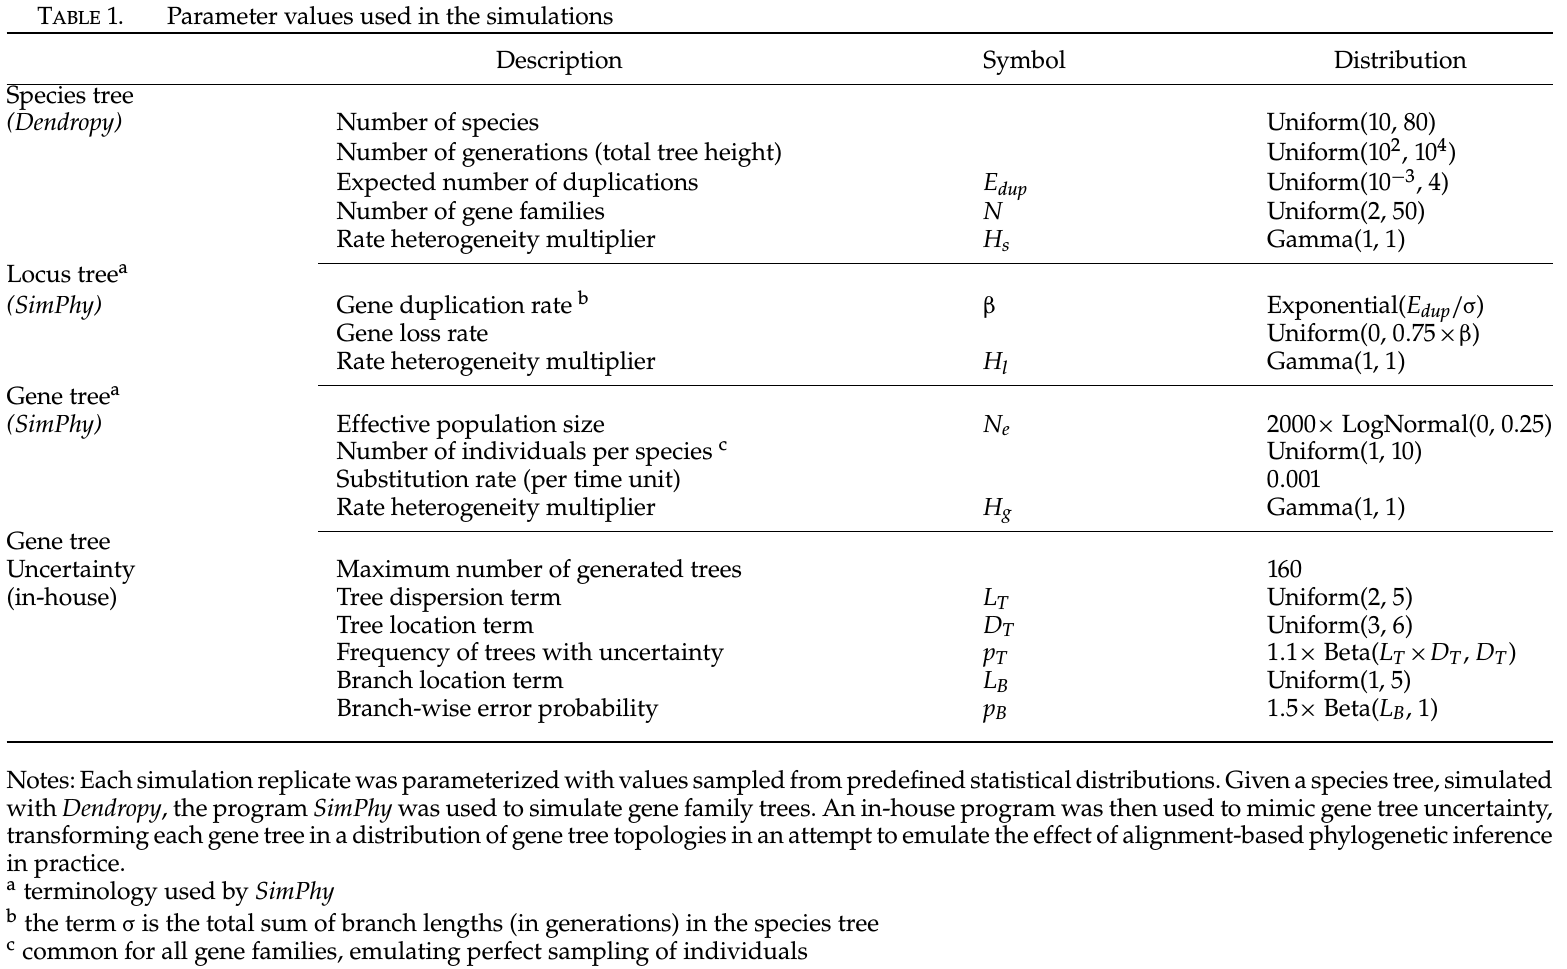
\includegraphics[scale=0.26]{table1.png}
\end{center}
}

%%%%%%%%%%%%%%%%%%%%%%%%%%%%%%%%%%%%%%%%%%%%%%%%%%%%%%%%%%%%%%%%%%%%%%%%%%%%%%%
\frame{
\begin{center}
 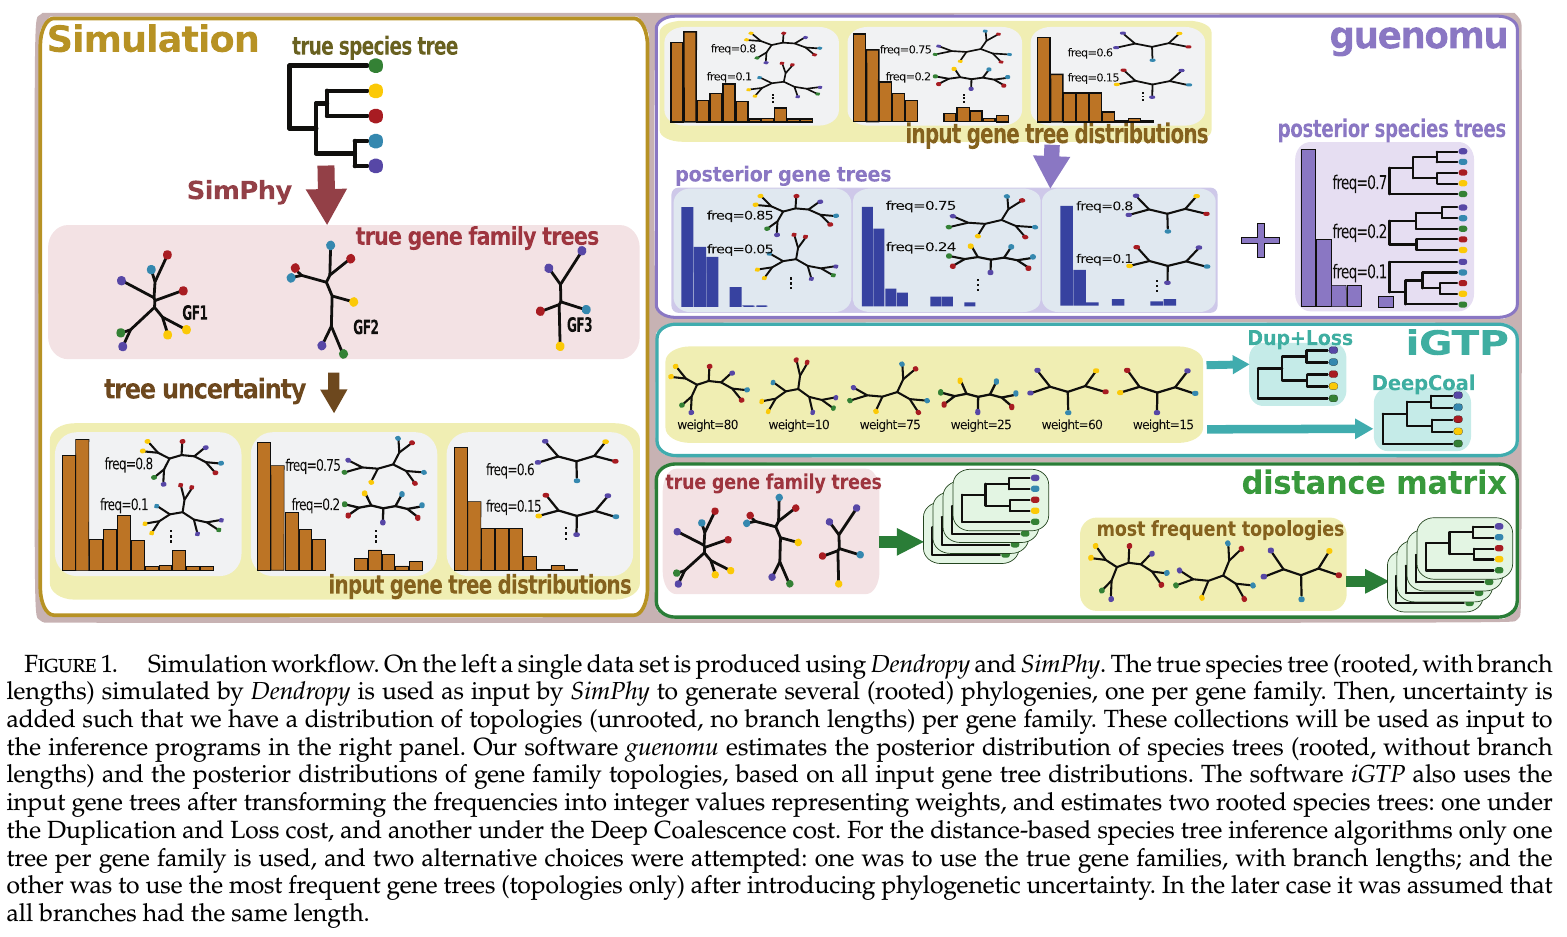
\includegraphics[scale=0.26]{figure1.png}
\end{center}
}

%%%%%%%%%%%%%%%%%%%%%%%%%%%%%%%%%%%%%%%%%%%%%%%%%%%%%%%%%%%%%%%%%%%%%%%%%%%%%%%
\section{Results}
\subsection{}
%%%%%%%%%%%%%%%%%%%%%%%%%%%%%%%%%%%%%%%%%%%%%%%%%%%%%%%%%%%%%%%%%%%%%%%%%%%%%%%

%%%%%%%%%%%%%%%%%%%%%%%%%%%%%%%%%%%%%%%%%%%%%%%%%%%%%%%%%%%%%%%%%%%%%%%%%%%%%%%
\frame{
\small
\frametitle{Notation}
\begin{itemize}
 \item DLI - a parameterization of the model that only considers reconciliation distances (min num. DL and ILS)
 \item DLIR - same except it also considers \textit{mulRF}
 \item iGTP - a competing software
\end{itemize}
\normalsize
}

%%%%%%%%%%%%%%%%%%%%%%%%%%%%%%%%%%%%%%%%%%%%%%%%%%%%%%%%%%%%%%%%%%%%%%%%%%%%%%%
\frame{
\begin{center}
 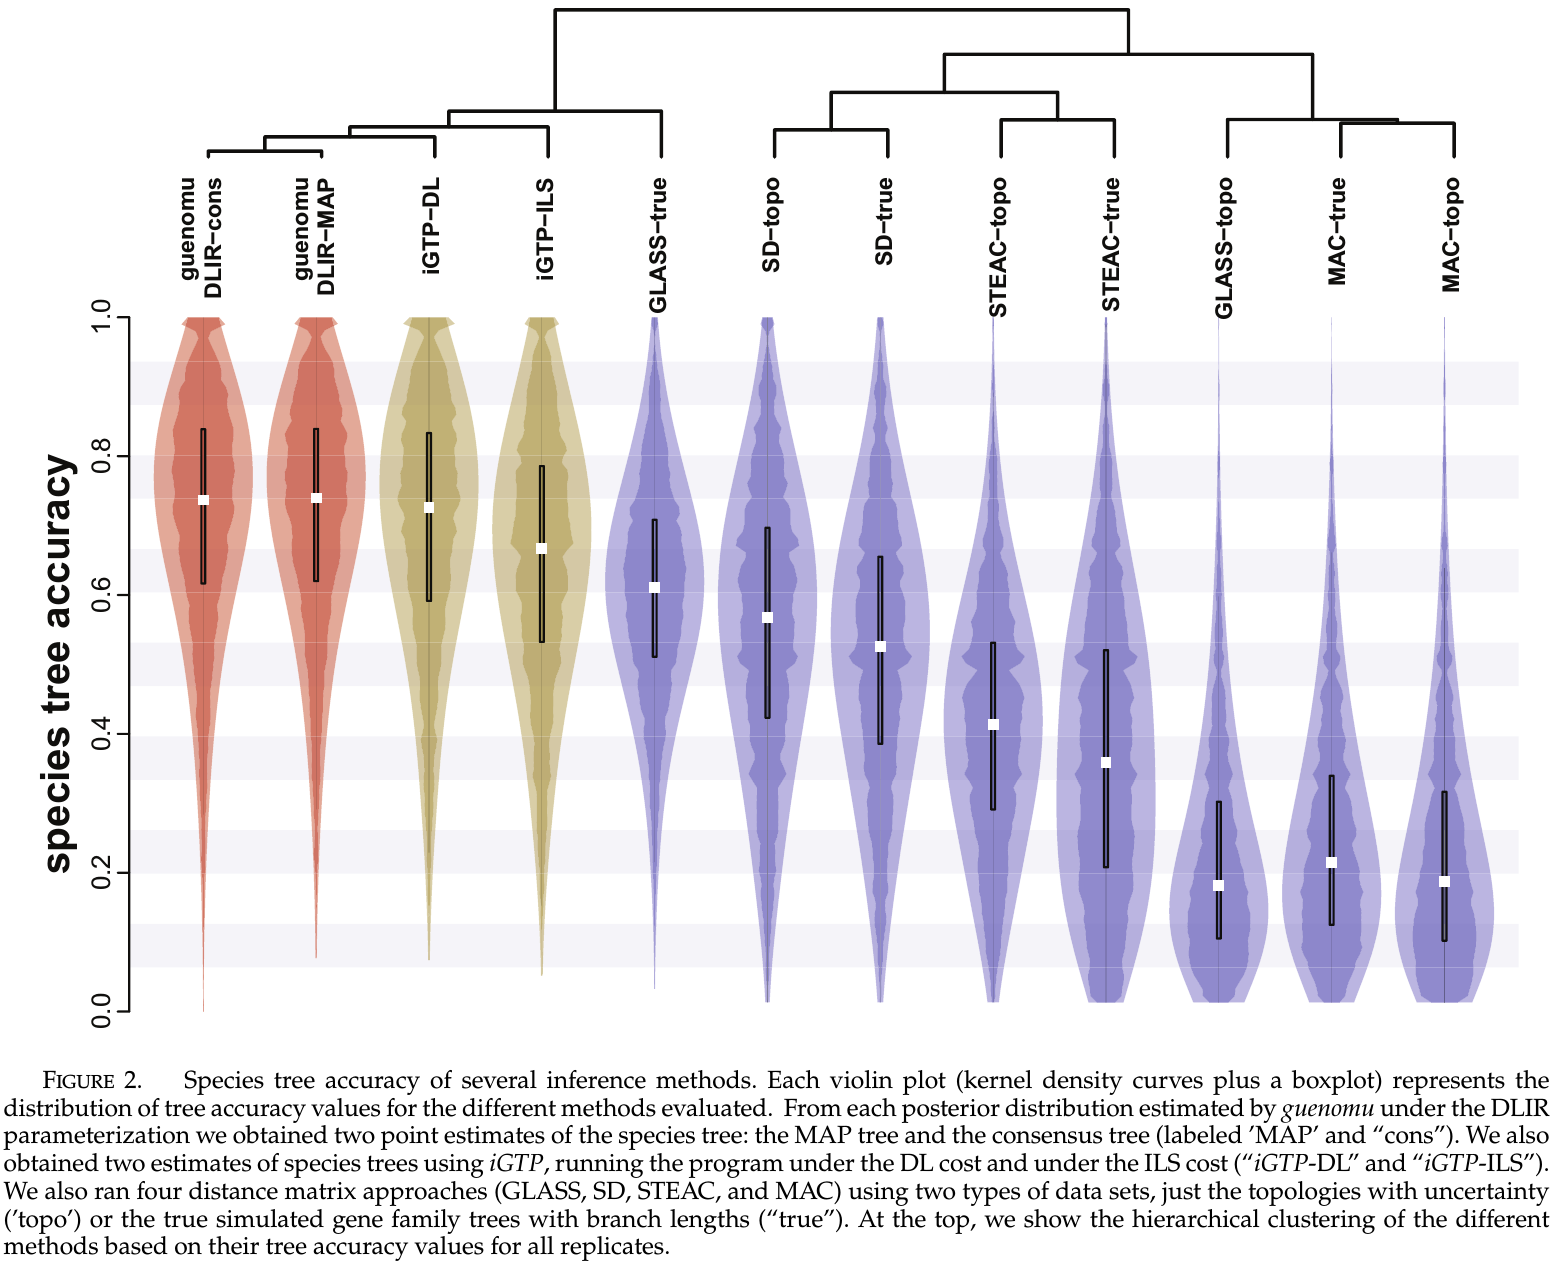
\includegraphics[scale=0.23]{figure2.png}
\end{center}
}

%%%%%%%%%%%%%%%%%%%%%%%%%%%%%%%%%%%%%%%%%%%%%%%%%%%%%%%%%%%%%%%%%%%%%%%%%%%%%%%
\frame{
\begin{center}
 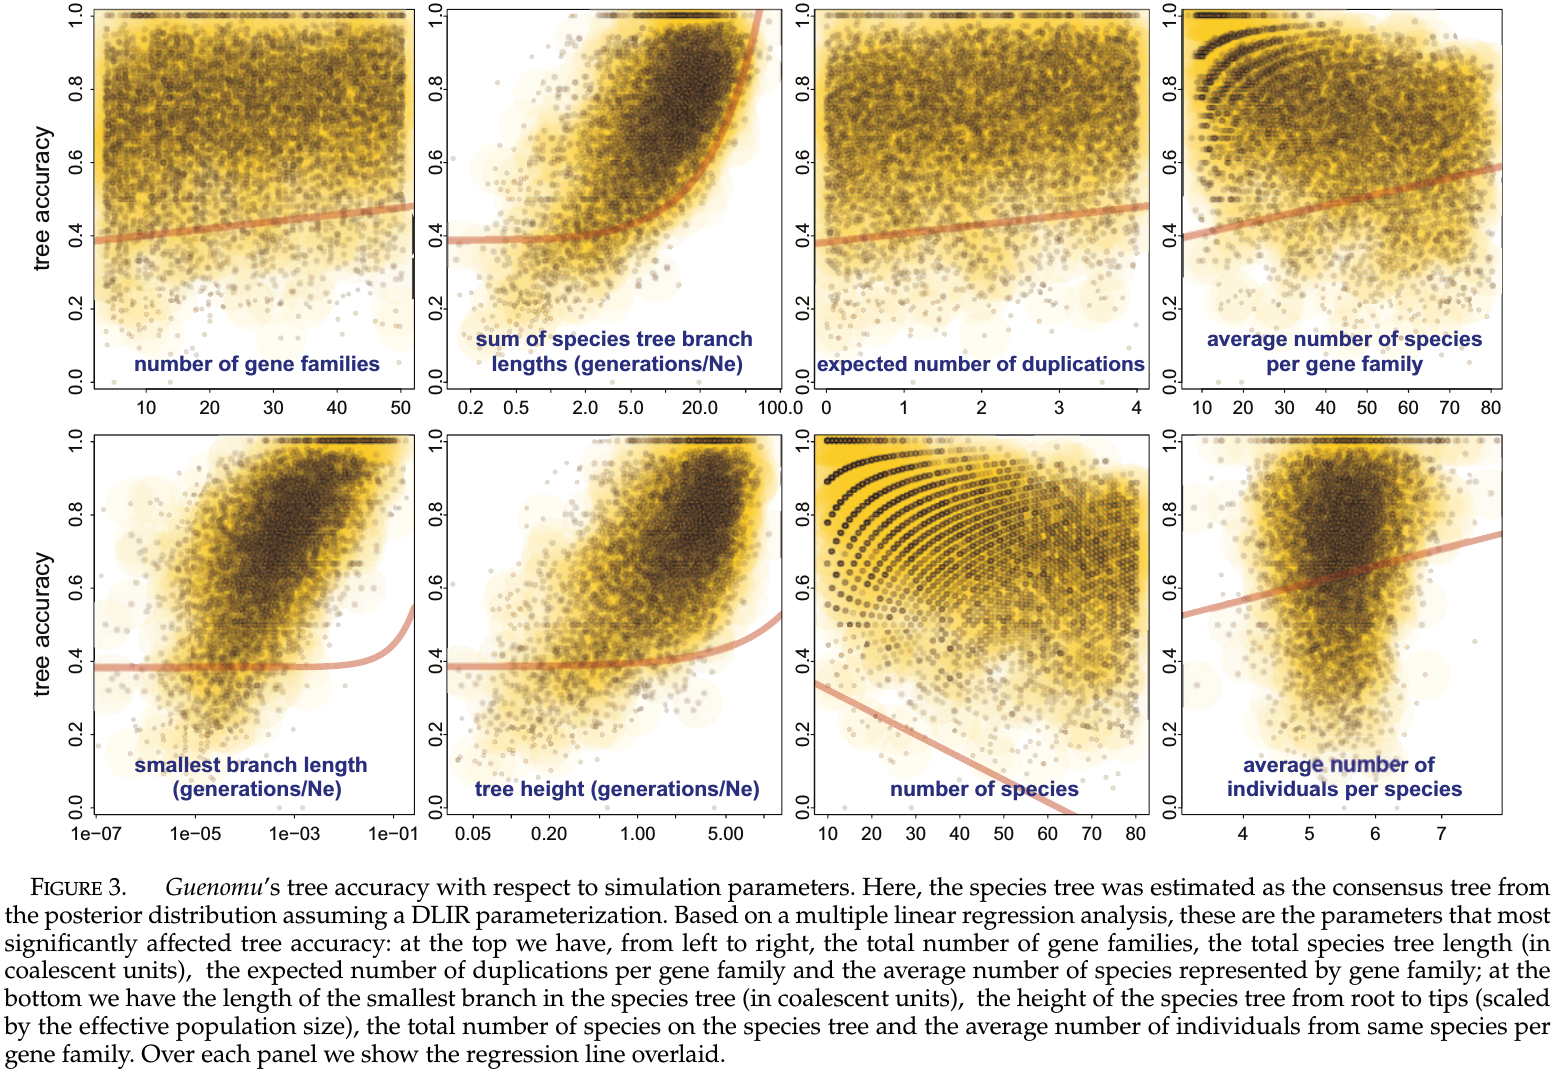
\includegraphics[scale=0.26]{figure3.png}
\end{center}
}

%%%%%%%%%%%%%%%%%%%%%%%%%%%%%%%%%%%%%%%%%%%%%%%%%%%%%%%%%%%%%%%%%%%%%%%%%%%%%%%
\frame{
\begin{center}
 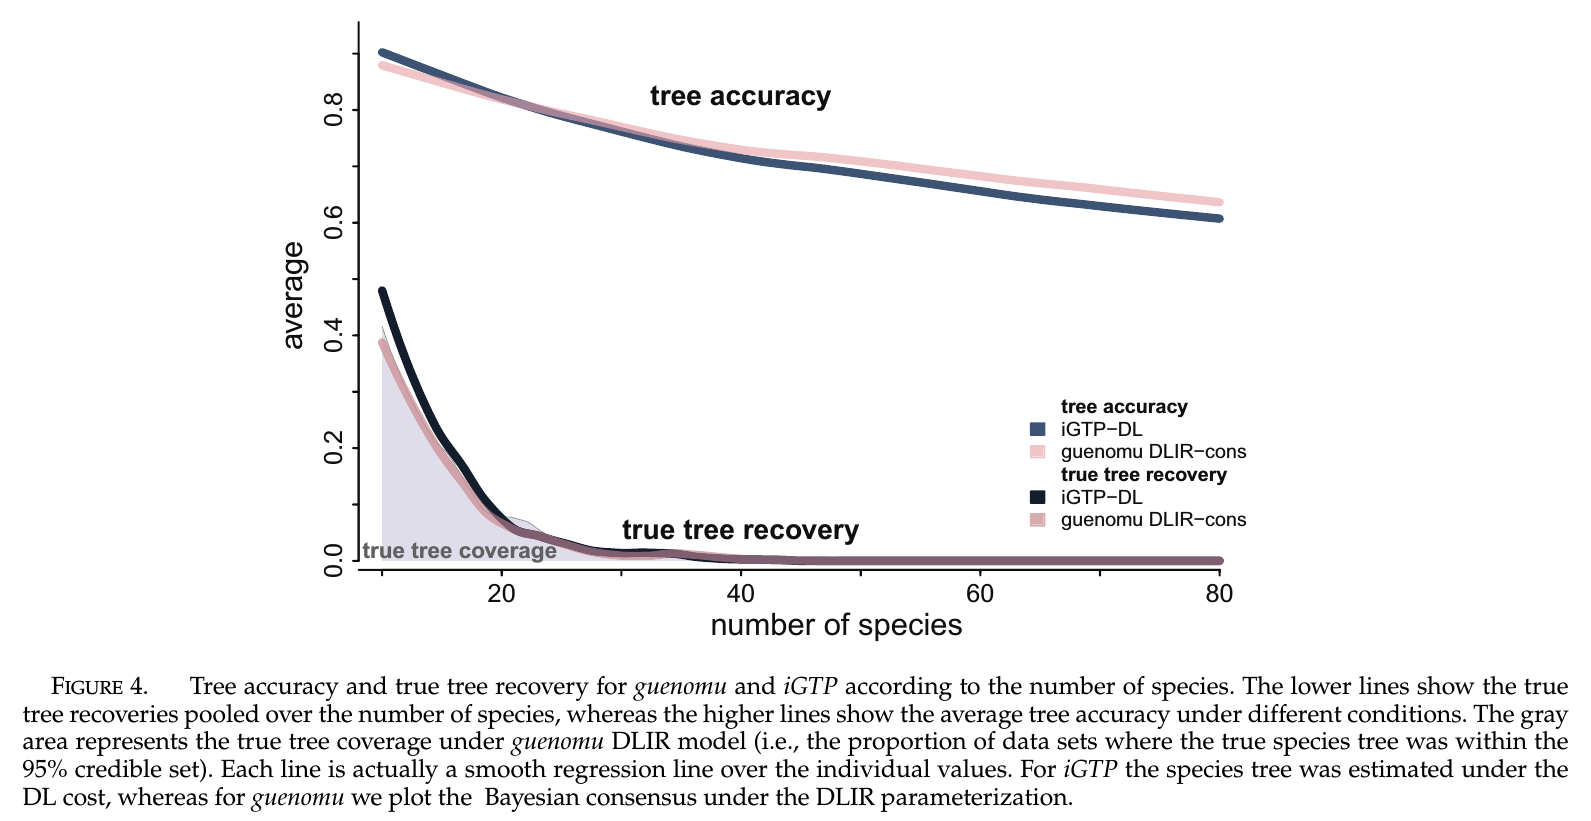
\includegraphics[scale=0.265]{figure4.png}
\end{center}
}

%%%%%%%%%%%%%%%%%%%%%%%%%%%%%%%%%%%%%%%%%%%%%%%%%%%%%%%%%%%%%%%%%%%%%%%%%%%%%%%
\frame{
\begin{center}
 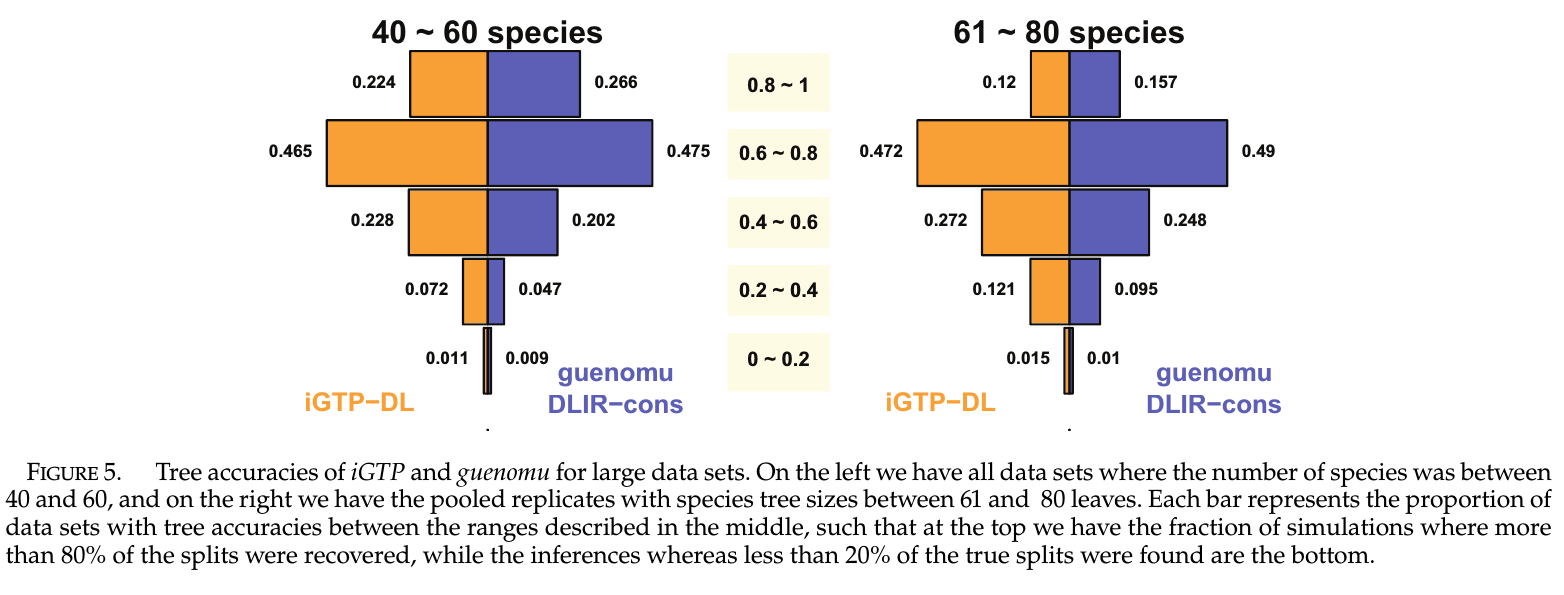
\includegraphics[scale=0.26]{figure5.png}
\end{center}
}

%%%%%%%%%%%%%%%%%%%%%%%%%%%%%%%%%%%%%%%%%%%%%%%%%%%%%%%%%%%%%%%%%%%%%%%%%%%%%%%
\frame{
\begin{center}
 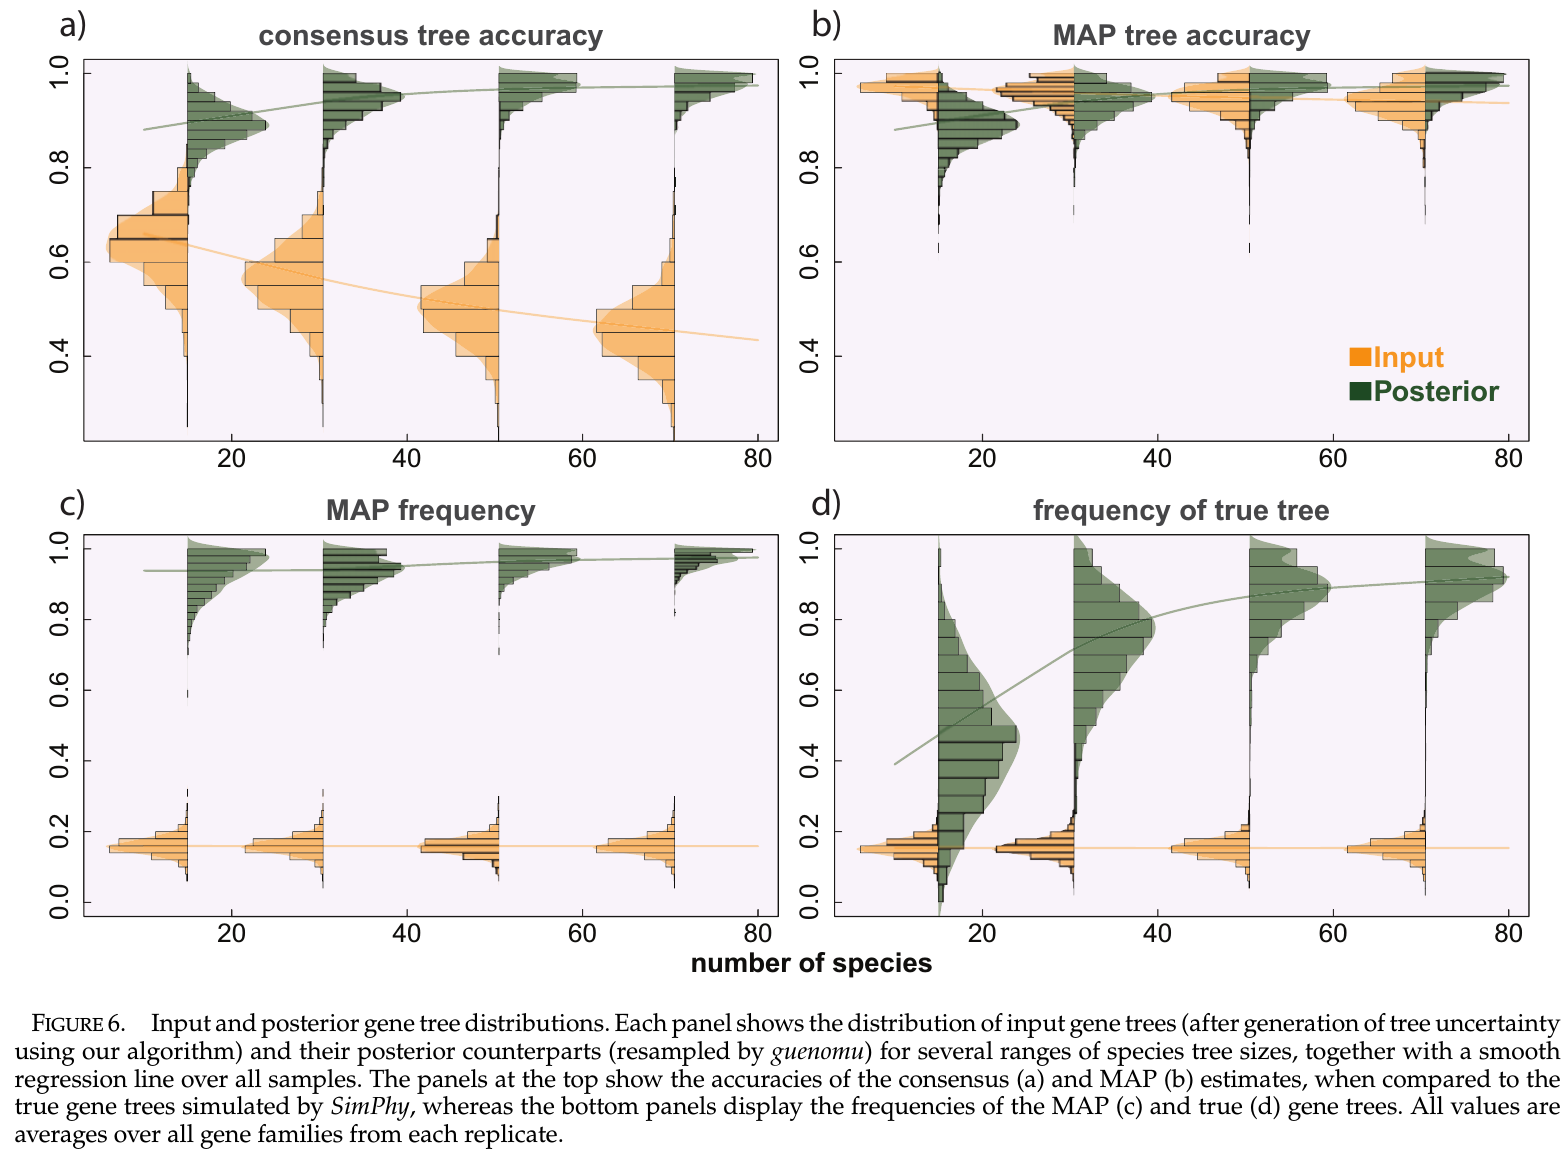
\includegraphics[scale=0.26]{figure6.png}
\end{center}
}

%%%%%%%%%%%%%%%%%%%%%%%%%%%%%%%%%%%%%%%%%%%%%%%%%%%%%%%%%%%%%%%%%%%%%%%%%%%%%%%
\section{Discussion}
\subsection{}
%%%%%%%%%%%%%%%%%%%%%%%%%%%%%%%%%%%%%%%%%%%%%%%%%%%%%%%%%%%%%%%%%%%%%%%%%%%%%%%

%%%%%%%%%%%%%%%%%%%%%%%%%%%%%%%%%%%%%%%%%%%%%%%%%%%%%%%%%%%%%%%%%%%%%%%%%%%%%%%
\frame{
\small
\begin{itemize}
 \item Usually different sources of gene tree disagreement are considered separately (e.g. DL,ILS), however unrecognized processes adversely affect gene tree estimation \cite{Rasmussen12}  
 \item guenomu does well, GTP methods do well, but coalescence methods perform poorly under the scenarios considered
\end{itemize}
\normalsize
}

%%%%%%%%%%%%%%%%%%%%%%%%%%%%%%%%%%%%%%%%%%%%%%%%%%%%%%%%%%%%%%%%%%%%%%%%%%%%%%%
\frame[allowframebreaks]{  
\tiny \bibliography{../../phylo-models.bib}
\bibliographystyle{apalike}          % Style BST file
}


%%%%%%%%%%%%%%%%%%%%%%%%%%%%%%%%%%%%%%%%%%%%%%%%%%%%%%%%%%%%%%%%%%%%%%%%%%%%%%%%
\end{document}